\section{Ajout d'un opérateur : gestion des préférences} \label{sec:valid:domvision:architecture}
Dans cette section, nous validons la flexibilité de notre architecture en intégrant un nouvel opérateur. De nombreux efforts ont été consacrés ces dernières années à la personnalisation des réponses lors de l'accès aux bases de données. Dans notre cadre, un de nos objectifs était de pouvoir adapter les résultats en fonction de l'utilisateur. Dans cette section, nous introduisons dans le cadre d'Astral-Astronef les opérateurs de \textit{CPref-SQL}~\cite{DeAmo:cprefsql}. Tout d'abord, nous présentons les notions théoriques nécessaires pour appréhender les préférences contextuelles. Puis, nous présentons les deux opérateurs permettant de sélectionner les n-uplets préférés sur une relation temporelle. Ensuite, nous appliquons ceci à notre cadre applicatif. Enfin, nous présentons comment l'intégration dans Astronef est faite.

\subsection{Préférences contextuelles}
Dans cette section nous présentons les principaux concepts concernant le formalisme logique que nous employons pour spécifier et raisonner avec des préférences. Tout d'abord présentons le concept de préférence contextuelle. Une \textit{préférence contextuelle} est une manière d'exprimer la phrase suivante : \enquote{\it Lorsque $u$ est vrai, je préfère $Q_1$ à $Q_2$ à attributs $W$ égaux}. La définition~\ref{def:pref} définie formellement cette notion.

\begin{defi}[Préférence Contextuelle]\label{def:pref}
Soit $A$ un ensemble d'attribut,

Une \textit{règle de préférence contextuelle} (ou \textit{cp-règle}) sur $A$ est une formule $\varphi$ de la forme :
 $$\varphi: u \rightarrow Q_1(X) \succ Q_2(X)\ [W]$$
\begin{itemize}
	\item $X$ est un attribut non-temporel de $R$ tel que $W \subseteq A$, $X \not \in W$,
	\item $Q_i(X)$ est une condition exprimée sur $X$,
	\item $\forall x$, $Q_1(x)$ et $Q_2(x)$ ne peuvent être satisfaites simultanément,
	\item $u$ est une condition ne portant ni sur $X$ ni sur les attributs de $W$.
	\end{itemize}
\end{defi}

La formule $u$ du côté gauche d'une cp-règle $\varphi$ est appelé son \textit{contexte}. L'expression $Q_1(X) \succ Q_2(X)$ du côté droit est appelé l' \textit{expression de préférence} et les attributs dans $W$ sont appelés des attributs \textit{ceteris paribus} (cf. ci-dessous). Un n-uplet $s$ est dit \textit{compatible} avec une cp-règle $\varphi$ si $s$ satisfait son contexte.

Une \textit{théorie de préférence contextuelle} (\textit{cp-théorie}) sur $A$ est un ensemble fini $\Gamma$ de cp-règles sur $R$. Nous notons par Attr($\Gamma$) l'ensemble d'attributs dans les cp-règles de $\Gamma$.

Ainsi, une cp-règle $\varphi$ sur $A$ induit une \textit{relation binaire} (notée $\succ_\varphi$) sur une séquence d'n-uplet d'attributs $A$, à savoir l'ensemble des paires ($s_1,s_2$) tels que $s_1$ est préféré à $s_2$ par rapport à $\varphi$. Cette relation binaire n'est pas nécessairement transitive, ce qui fait que ce n'est pas une \textit{relation d'ordre}. Nous définissons la notion de \textit{Relation de Préférence} inférée par une cp-théorie $\Gamma$.

\begin{defi}[Relation de Préférence]
Soit $\Gamma$ cp-théorie sur $A$,

La \textit{Relation de Préférence} associée à $\Gamma$ (notée $\succ_\Gamma$) est définie comme :
\begin{center} $\succ_\Gamma = (\cup_{\varphi \in \Gamma} \succ_\varphi)^*,$ o\`u $*$ dénote la \textit{fermeture transitive}.\end{center}
\end{defi}

Cette relation de préférence est dites \textit{consistante} si et seulement si elle est irréflexive. Si tel est le cas, elle devient ainsi une relation d'ordre partielle stricte. Des travaux existent pour vérifier si une cp-théorie est consistante~\cite{Wilson:cpnet}. Nous supposons pour la suite du document que nos relations le sont.

\subsection{Opérateurs de Préférences}
Les opérateurs de préférences calculent les données préférées par rapport à une cp-th\'eorie de référence. Chaque utilisateur donne au système ses préférences sous forme d'une cp-th\'eorie $\Gamma$ qui constitue ainsi une sorte de \textit{profil utilisateur} qui est évolutif. Concrètement, cette solution va permettre le support de requêtes 
\enquote{les plus préférées} et \enquote{les top-k} par l'intégration de deux opérateurs: \textbf{Best} et \textbf{KBest}.

L'opérateur \textbf{Best} sélectionne, dans relation temporelle ou non-temporelle, les n-uplets qui correspondent le mieux à l'ensemble des préférences représentés dans $\Gamma$. D'un point de vue mathématique, il s'agit des n-uplets qui ne sont pas dominés dans la hiérarchie des préférences.

\begin{defi}[Best]\label{def:best}
Soit $R$ une relation temporelle et $\Gamma$ une cp-th\'eorie sur le schéma de $R$. 

\textbf{Best}$(R): b\mapsto \{u \in R(b) \mid \not\exists v \in r(t) \textrm{ tel que } v \succ_\Gamma u \}$
\end{defi}

L'opérateur \textbf{KBest} sélectionne les $k$ n-uplets qui correspondent au mieux à la hiérarchie des préférences énoncées dans $\Gamma$. Intuitivement \textbf{KBest}$_k(R)(b)$ retourne l'ensemble des $k$ n-uplets de $R(b)$ qui sont le moins dominés par d'autres n-uplets selon la hiérarchie de préférences. Pour définir sa sémantique nous introduisons la notion de \textit{niveau} d'un n-uplet (notée $l(u)$) par rapport à une cp-théorie $\Gamma$ dans la définition~\ref{def:niveau}. Le niveau reflète l'écart entre ce n-uplet et ceux qui répondent complètement aux préférences de l'utilisateur.

\begin{defi}[Niveau]\label{def:niveau}
Soit $R$ une relation temporelle et $\Gamma$ une cp-th\'eorie sur le schéma de $R$.

Le \textit{niveau} de $u$, $l(u)$, \textit{par rapport à} $\Gamma$ au \textit{batch} $b$ est définie de manière inductive comme suit:
 \begin{itemize}
 \item Si $\not\exists u' \in R(b)$ tel que $u' \succ_\Gamma$ $u$, alors $l(u) = 0$.
 \item sinon $l(u)$ = $1+max \{l(u') \mid u' \succ_\Gamma u\} $
 \end{itemize}
\end{defi}

Il est possible de montrer que si $u \succ u'$ alors $l(u) < l(u')$. La réciproque n'est pas vraie. La sémantique de l'opérateur \textbf{KBest}$_k$ est présenté dans la définition~\ref{def:kbest}.

\begin{defi}[KBest]\label{def:kbest}
Soit $R$ une relation temporelle et $\Gamma$ une cp-th\'eorie sur le schéma de $R$. 

Pour un batch donné $b$, \textbf{KBest}$_k(R)(b)$ est l'ensemble des $k$ tuples $\in R(b)$ ayant le plus petit niveau. L'ordre positionel est utilisé pour départager des n-uplets de même niveau.
\end{defi}

\subsection{Exemple de requête}
Supposons l'existence d'un flux $V$ agrégeant l'ensemble des informations \textit{volatiles}. Son schéma est le suivant : $V$(id, concept, type, volatile, value, $\t$). La description de ce schéma est l'expression suivante : l'entité de nature \textit{concept}, d'identifiant \textit{id} et de catégorie \textit{type} a émit la donnée de type \textit{volatile} et de valeur \textit{value} au temps $\t$. La formation de ce flux est triviale selon les principes développés en section~\ref{sec:valid:domvision:requetes} et n'est pas détaillé.

Nous souhaitons utiliser ce flux en tant que flux d'information à afficher à l'utilisateur. Afin de rapidement analyser l'activité du réseau, il souhaite obtenir une sélection des meilleures informations le concernant.

Soit $\Gamma$ la cp-théorie comportant les préférences contextuelles suivantes :
\begin{itemize}
	\item $\varphi_1 : $ volatile = cpu $\mapsto ($value $ \geq 90) \succ ($value $ < 90)$ [id]
	\item $\varphi_2 : $ $($volatile = status$) \succ ($volatile = cpu $ \vee $ volatile = mem$)$ [type]
	\item $\varphi_3 : $ concept = interface $\mapsto ($type = wifi$) \succ ($type = ethernet$)$
\end{itemize}

La figure~\ref{fig:valid:domvision:architecture:pref} représente un ensemble de données pour $V$. Si nous appliquons la relation d'ordre sur cet ensemble d'n-uplet, nous pouvons remarquer que par la règle $\varphi_1$, nous obtenons que $s_1 > s_4$. Par $\varphi_2$ nous obtenons que $s_2 > s_1$. Et enfin, nous avons $s_3 > s_5$ par $\varphi_3$. La relation d'ordre $\succ_\Gamma$ est transitive, ainsi $s_2 > s_4$. Le graphe de la figure représente ces relations d'ordres.
\begin{figure}[ht]\centering
\begin{tabular}{|c|c|c|c|c|c|c|} \bottomrule
\rowcolor{hypcolor} $V$ & id & concept & type & volatile & value & $\t$\\ \hline
$s_1$ & 1 & equipement & gateway & cpu & 95 & 1\\ \hline % 1 > 4
$s_2$ & 2 & equipement & stb & status & 1 & 2\\ \hline % 2 > 1 > 4
$s_3$ & 3 & interface & wifi & bws & 150 & 3\\ \hline %
$s_4$ & 1 & equipement & gateway & cpu & 20 & 4\\ \hline
$s_5$ & 5 & interface & ethernet & bwr & 1200 & 5\\ \toprule % 3 > 5
\end{tabular}\hspace{1cm}
\begin{minipage}{3cm}
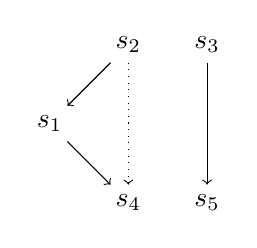
\begin{tikzpicture}[<-]
\node (sb) at (1,2) {$s_2$};
\node (sa) at (0,1) {$s_1$} edge (sb);
\node (sd) at (1,0) {$s_4$} edge (sa);

\draw (sd) edge [dotted] (sb);

\node (sc) at (2,2) {$s_3$};
\node (se) at (2,0) {$s_5$} edge (sc);
\end{tikzpicture}
\end{minipage}
\caption{Un jeu de données pour $V$ et son graphe de préférence correspondant}\label{fig:valid:domvision:architecture:pref}
\end{figure}

En supposant que nous appliquons une fenêtre sur $V$ et que nous obtenons les n-uplets présentés au batch $b$. Nous obtenons les résultats suivant : 
\begin{itemize}
	\item \textbf{Best}$(R)(b) = \{s_2,s_3\}$, car ces deux n-uplets ne sont pas dominés.
	\item \textbf{KBest}$_3(R)(b) = \{s_1,s_2,s_3\}$ par sélection du niveau 0 et 1.
	\item \textbf{KBest}$_4(R)(b) = \{s_1,s_2,s_3,s_4\}$, car $s_5$ est arrivé après $s_4$ et l'ordre positionnel domine à niveau équivalent.
\end{itemize}

Dans la pratique nous pourrions appliquer cet opérateur sur tout type de fenêtre. Pour revenir à notre application, en supposant que $V$ est correctement formé, nous pouvons déployer une requête continue qui peut alimenter l'interface de l'utilisateur avec : les 25 événements les plus importants du dernier jour évalué toutes les minutes. Cette requête a l'expression $\textbf{KBest}_{25}(V[T\ 1j\ 1min])$.

\subsection{Intégration dans Astronef}
Nous avons désormais des définitions Astral correctement posées. Nous pouvons maintenant intégrer ces opérateurs à Astronef. En premier lieu, nous avons conçu un composant opérateur capable de calculer les sémantiques de \textbf{Best} et \textbf{KBest} de manière statique en calculant à partir de l'état de $R(b)$. Ce composant prend évidemment en paramètre $k$ qui peut être égal à $-1$ pour indiquer une sémantique de \textbf{Best}.

L'intégration du composant se fait en deux parties. Tout d'abord, il est nécessaire d'enregistrer le composant en tant qu'opérateur, ceci est fait automatiquement lorsque le binaire est installé. Ensuite, il faut renseigner ses définitions Astral dans le moteur de règle. Dans notre cas, quatre règles sont suffisantes :
\begin{lstlisting}
sugar([best,Config,C],[kbest,NewConfig,C]):-
    map_put(Config,['k',-1],NewConfig), !. % best = kbest avec k=-1

typerules([kbest,_,_,[T]],T):- relation(T), !.
attribrules([kbest,_,_,[A]], A):- !.

implrules([kbest,_,_,_], "KBest"):- !.
\end{lstlisting}

Une fois ce code renseigné dans le service de connaissance d'Astronef, nous pouvons librement utiliser les opérateurs \textbf{Best} et \textbf{KBest} sur toutes relations temporelles. Nous avons aussi développé un composant similaire mais dont l'algorithme est calculé de façon incrémental. Maintenant que les définitions des opérateurs sont renseignés, son intégration est simplifiée avec deux règles :
\begin{lstlisting}
dynamicoperator([kbest,B,[C]]):- !,
    map_get(B, "incremental", "true", "true"), % Mode incremental par defaut
    dynamicoperator(C). % Si le noeud fils est aussi incremental

implrules([kbest,B,_,_], "DynamicKBest"):- isdynamic(B), !.
\end{lstlisting}

Nous verrons l'implémentation de ces algorithmes dans le chapitre~\ref{chap:validation:perfs} ainsi qu'une étude sur le choix de l'un ou l'autre algorithme. Il est intéressant de voir que si le SGBD supporte le langage \textit{CPref-SQL}, nous pouvons pousser les opérateurs \textbf{Best} et \textbf{KBest} sur le SGBD via une règle Asteroid. 